\section{内存管理}

内存 (RAM) 是计算机中不可缺少的重要硬件,所有程序的运行都是在内存中进行的,
而CPU访问硬盘数据也必须先经过内存交换才得以实现,内存在加速CPU访问硬盘居功至伟。
由内存的重要性可知内存管理在操作系统中也非常重要。	

由于内存在计算机整体架构中的特殊性,内存错误将导致程序或操作系统错误,后果非常严重。
故操作系统在计算机启动后需要检查内存,确保内存未发生故障,
然后初始化内存并清空内存空间,在程序发出内存申请后才向其分配内存,
并在程序运行结束后释放其内存。

功能设计如图~\ref{fig:memman}所示。
\begin{figure}[H]
  \centering
  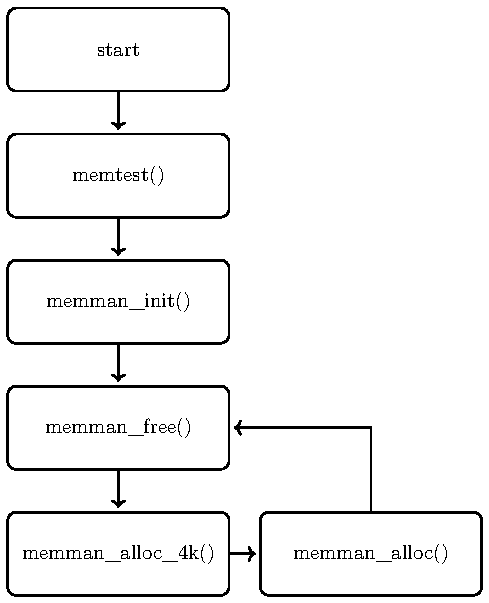
\includegraphics[width=.5\textwidth]{../Fig/func/memman.pdf}
  \caption{内存管理}
  \label{fig:memman}
\end{figure}

\begin{description}
  \csingle|unsigned int memtest(unsigned int start, unsigned int end);|
  \begin{itemize}
    \item 检测整个内存并返回可用内存大小;
  \end{itemize}
  \csingle|void memman_init(struct MEMMAN *man);|
  \begin{itemize}
    \item 初始化各内存块,并初始化块信息;
  \end{itemize}
  \csingle|int memman_free(struct MEMMAN *man, unsigned int addr, unsigned int size);|
  \begin{itemize}
    \item 释放指定大小的内存地址空间;
  \end{itemize}
  \csingle|unsigned int memman_alloc_4k(struct MEMMAN *man, unsigned int size);|
  \begin{itemize}
    \item 分配指定大小的内存空间;\\
  \end{itemize}
\end{description}

内存的结构通常用地址和空间表示,在计算机运行过程中,
内存的分配是随机的,导致内存的释放也是相对无序的,这样导致了很多的碎片化问题,
也就是随计算机运行时间变长,内存中到处遍布小块零散空闲空间,虽然零散空间总数很大,
但很难满足新进程序的内存需求,于是内存管理显得十分必要。

内存管理设计的主要目的是快速并且高效的分配内存空间,并在适当的时间释放并回收内存空间。
根据内存管理的设计目的,数据结构设计参见程序~\ref{lst:mem}。

\begin{listing}[H]
  \inputminted[tabsize=2, firstline=137, lastline=143,
    linenos=true]{c}{../ZOS/src/kernel/bootpack.h}
  \caption{数据结构-内存管理}
  \label{lst:mem}
\end{listing}

\begin{description}
\item[frees:]当前可用内存组数;
\item[maxfrees:]可用内存组数的最大;
\item[lostsize:]释放失败的内存的大小总和;
\item[losts:]释放失败次数。
\end{description}

经过内存初始化和释放所有内存空间后,内存管理正常运行。

\subsection{内存分配}

内存的分配方式涉及到内存释放的效率,好的分配方式会使得内存使用的效率大大提高。
根据内存的大小来组织内存的使用方式,预计使用32KB用于内存分配的管理空间,
则共有4000组左右的内存用于分配给各个程序使用,每个组4KB。

每一组内存经过初始化都拥有自己的数据结构,
即每一组空闲内存的地址和大小都被记录到空闲内存表,如表~\ref{tab:free}所示。

\begin{table}[h]
  \centering
  \begin{tabular}{ccc}
    \hline
    组号 & 地址 & 大小 \\\hline
    2 & 0x00005000 & 1000 \\
    1 & 0x00004000 & 1000 \\
    0 & 0x00003000 & 1000 \\\hline    
  \end{tabular}
  \caption{空闲内存表free}
  \label{tab:free}
\end{table}

程序向操作系统发出申请内存的请求(需求的内存大小),
操作系统收到请求后开始在空闲内存组中寻找足够大的连续内存完成这次申请,并返回可供使用的空闲内存的地址和大小。

完成申请后系统需要重新整理空闲内存表free,将可用内存组数减一,
将返回给程序空闲空间大小根据程序需求进行调整,并对剩余的可用内存表进行按地址升序整理。

代码参见程序~\ref{lst:alloc}。

% ----------------------------

\subsection{内存释放}

为保证磁盘空闲空间尽可能少的碎片化,内存释放首先考虑的是使待释放空间与附近空闲空间进行合并\cite{bryant2003computer}。

具体分为三种情况:

\begin{description}
\item[前端空闲:]释放内存的相连前端是空闲内存或释放内存相连两端都是空闲内存;
\item[后端可用:]释放内存的相连后端是空闲空间;
\item[前端后端均不可用:]在当前位置释放内存。
\end{description}

\newpage

已知:待释放的空间的地址和空间大小。

根据空闲内存表free的编号从0到frees遍历查找地址大于待释放空间的空闲内存,
并根据得到的空闲内存编号i及大小size区分此时的待释放内存应当采取何种方式释放,实现参见附录程序~\ref{lst:rw}。

\subsubsection{前端空闲}

释放内存时,当待释放空间的相连前端有可用内存时,将可释放内存大小归入前端可用内存内,frees不变;

当相连后端也有可用内存时,将后端内存大小归入前端可用内存内,frees减一。

内存释放前后情况如图~\ref{fig:mem0}和图~\ref{fig:mem1}所示,实现参见附录程序~\ref{lst:mem1}所示。

\begin{figure}[H]
  \centering
  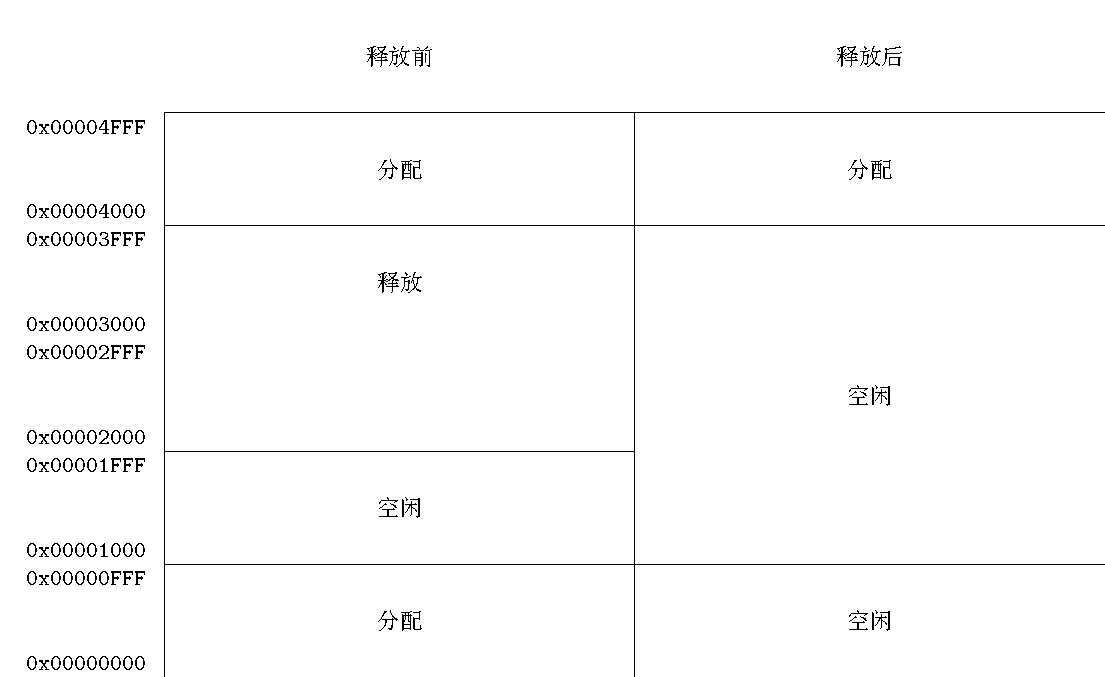
\includegraphics[width=.7\textwidth]{../Fig/mem0.pdf}
  \caption{前端空闲}
  \label{fig:mem0}
\end{figure}

\begin{figure}[H]
  \centering
  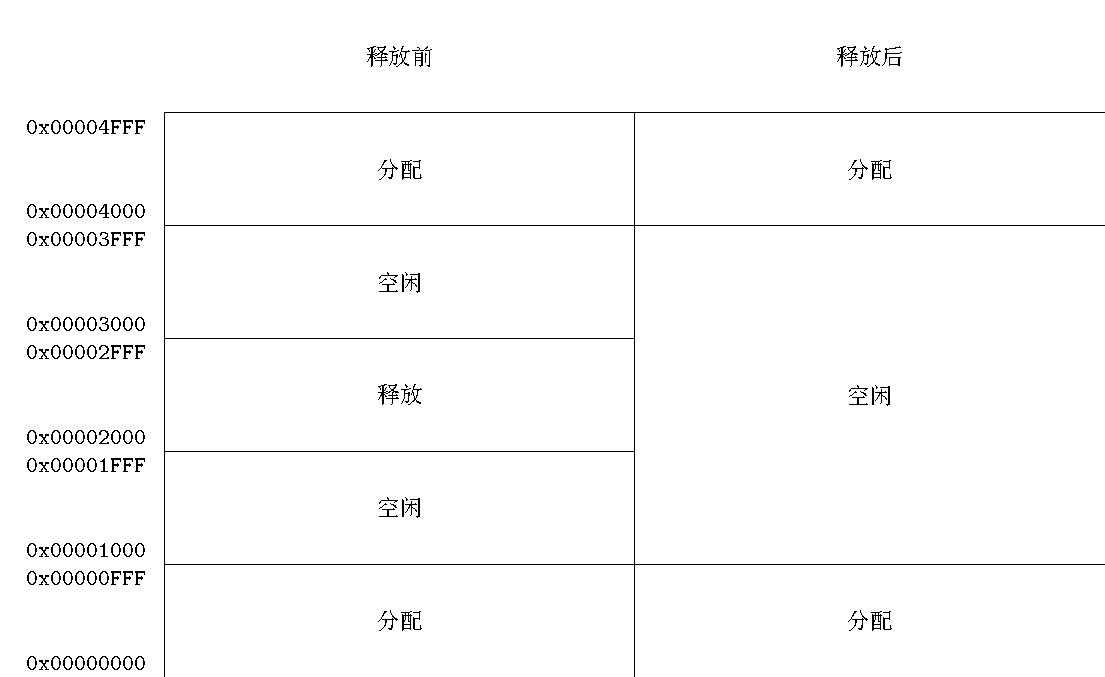
\includegraphics[width=.7\textwidth]{../Fig/mem1.pdf}
  \caption{前端可用,且后端空闲}
  \label{fig:mem1}
\end{figure}

% ------------------------------

\subsubsection{后端空闲}

释放内存时,当待释放空间的当相连后端有可用内存的时候将free[i]的地址换为待释放内存的地址,相连后端内存大小归入待释放内存大小,frees不变。

内存释放前后情况如图~\ref{fig:mem2}所示,实现参见附录程序~\ref{lst:mem2}所示。

\begin{figure}[H]
  \centering
  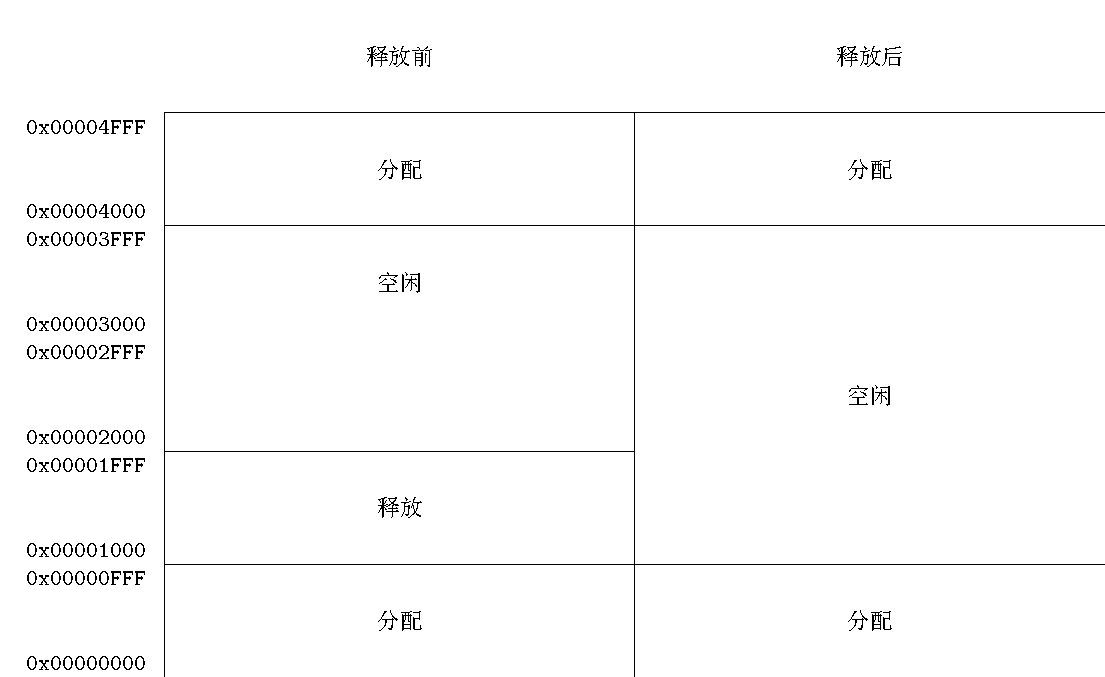
\includegraphics[width=.7\textwidth]{../Fig/mem2.pdf}
  \caption{后端空闲}
  \label{fig:mem2}
\end{figure}

% -----------------------------

\subsubsection{前端后端均被占用}

由于被释放空间周围没有空闲内存,为保证free内各段内存仍然按照内存地址升序排列,
使空闲空间计数最大值加一,free[i]后续空闲内存序号加一,并将释放空间组号定为i。

内存释放前后情况如图~\ref{fig:mem3}所示,代码参见附录程序~\ref{lst:mem3}。
\begin{figure}[H]
  \centering
  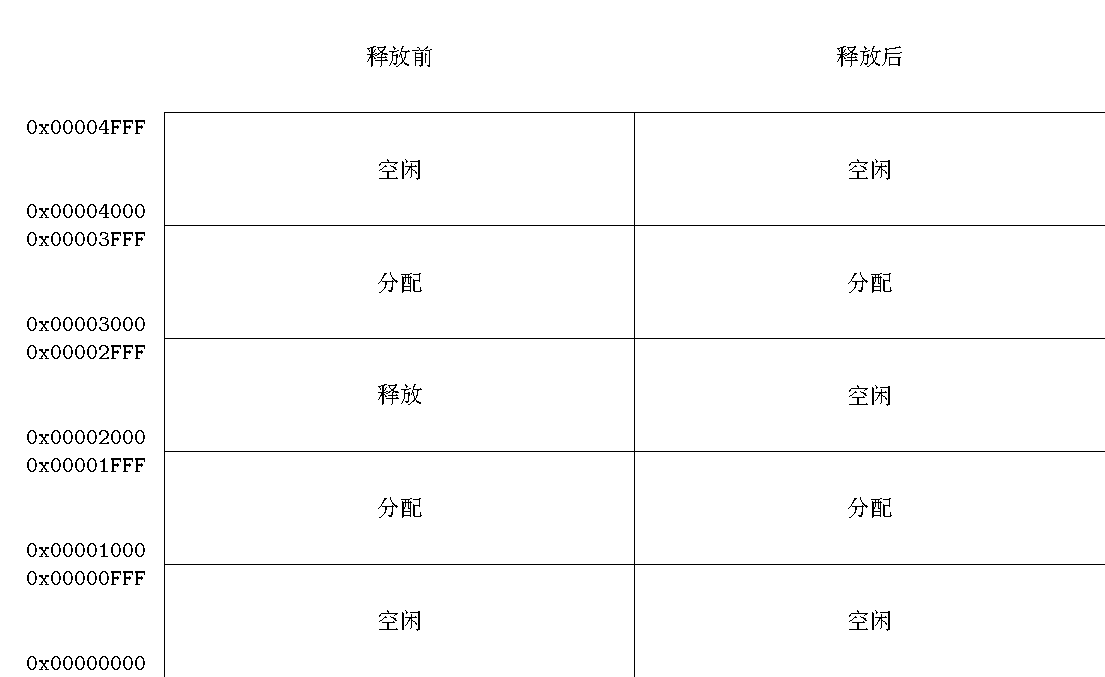
\includegraphics[width=.7\textwidth]{../Fig/mem3.pdf}
  \caption{前端后端均被占用}
  \label{fig:mem3}
\end{figure}

% \subsubsection{小结}
% 经过合理的内存释放,计算机在使用一段时间后,内存中仍然保留着一部分大的空闲内存空间。